\documentclass{beamer}
\usepackage{graphicx}
\usepackage{amssymb,amsfonts,amsmath}
% \usepackage{tikz,tkz-euclide}
\usepackage{subcaption}
% \usepackage{parskip}
% \usetikzlibrary{arrows.meta}
% \usetikzlibrary{calc,patterns}
\usefonttheme[onlymath]{serif}
% \usetheme{Berlin}
\title{Weekly Report}
\author{WU Zihan}
\begin{document}
\maketitle
\begin{frame}
    \frametitle{Outline}
    \tableofcontents
\end{frame}

\section{Method for Noisy Data}
\begin{frame}
    \frametitle{Method for Noisy Data}
    $S_{\text{th}}$ denotes the thereshold for finding a co-cluster in a submatrix;
    $T_p$ denotes the times of reparitioning.
    \begin{itemize}
        \item Step 1: Decide $S_{\text{th}}$ with confidence level $1 - \beta_1$
        \item Step 2: Decide $T_p$ with confidence level $1 - \beta_2$
        \item $p = (1 - \beta_1)(1 - \beta_2) \ge 1 - (\beta_1 + \beta_2)$
        \item Select $\beta_1 = \beta_2 = 0.005$, then $p \ge 0.99$
    \end{itemize}
\end{frame}

\section{Experiment Results on Noisy Data}
\begin{frame}
    \frametitle{Results on Noisy Data}
    % two columns
    \begin{columns}
        \begin{column}{0.5\textwidth}
            \textbf{Settings}
            % smaller font
            \scriptsize
            \begin{itemize}
                \item $M = N = 10^4$
                \item $M_k = N_k \in \{50, 60, \dots, 190\}$
                \item $\kappa = \cfrac{\sigma^2}{B_{\max}} \in \{0.001 , 0.005, 0.01, 0.05, 0.1\}$
            \end{itemize}
            \textbf{Results}
            % figure result.png
            \begin{figure}[htb]
                \centering
                
\includegraphics[width=\linewidth]{result.png}
                \caption{Results on Noisy Data}
                \label{fig:results}
            \end{figure}
        \end{column}
        \begin{column}{0.5\textwidth}
            \vspace{-1cm}
            \centering
            \begin{figure}[htb]
                \centering
                \begin{subfigure}[b]{\textwidth}
                    \centering
                    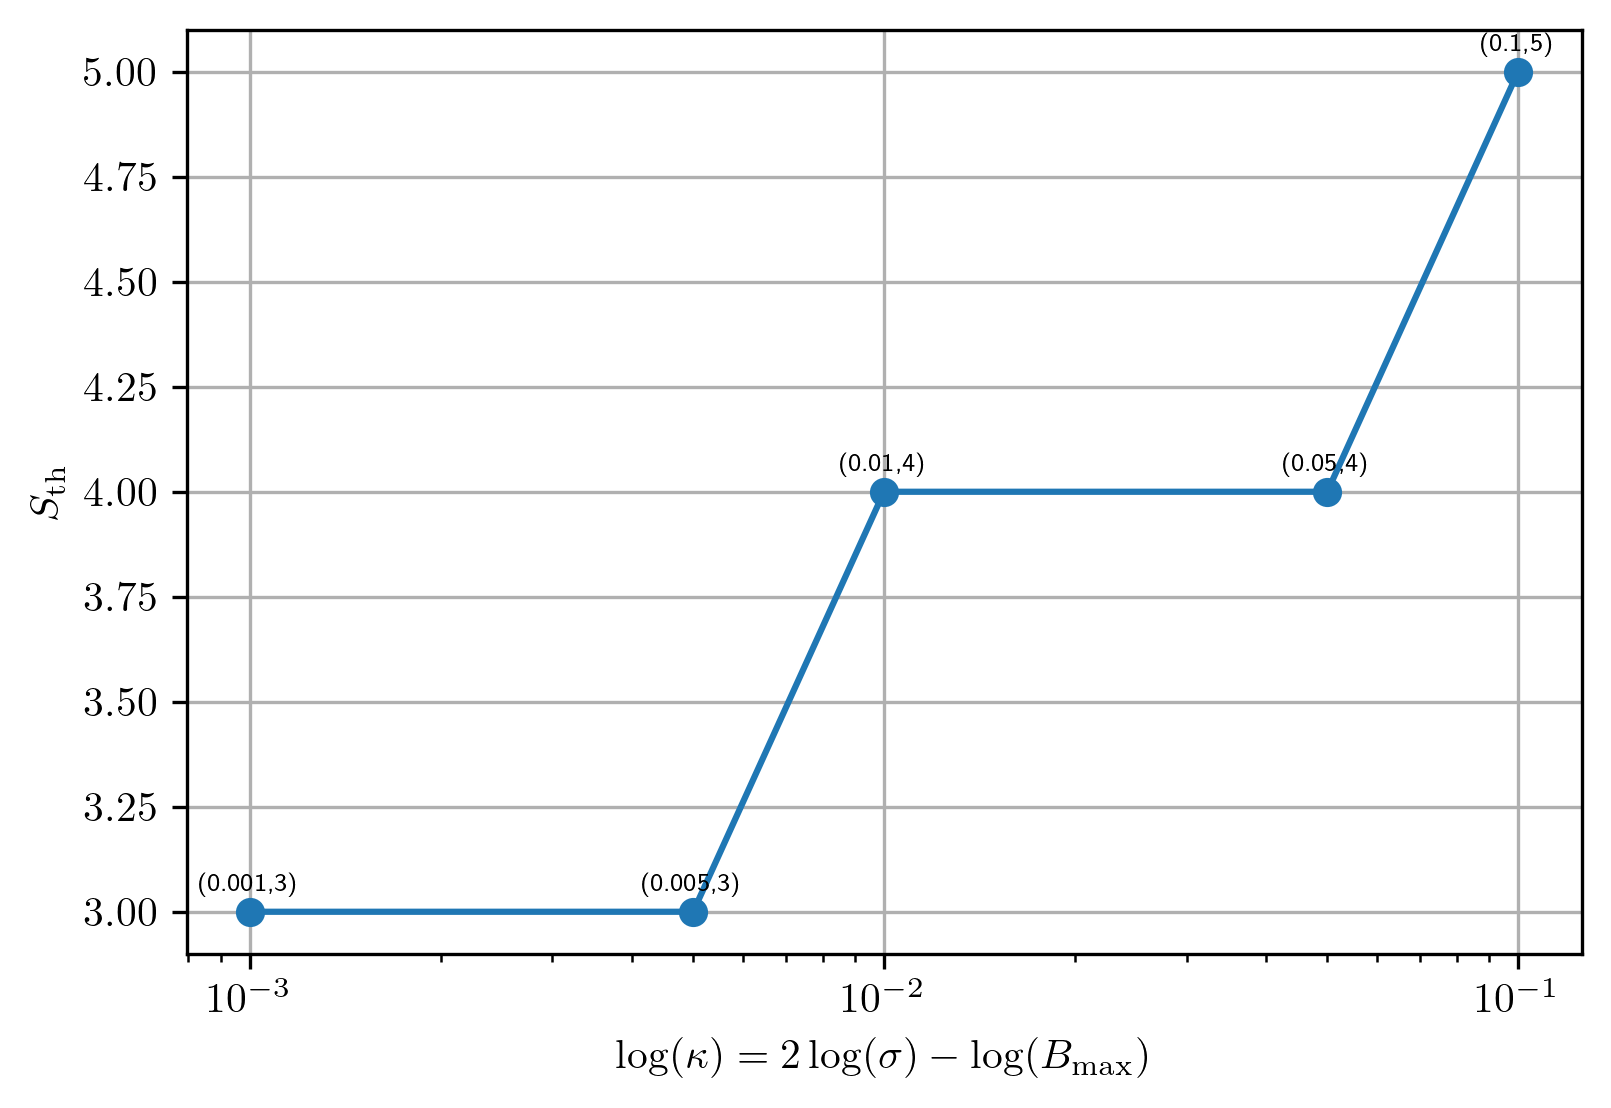
\includegraphics[width=\linewidth]{Tm.png}
                    \caption{Decide $S_{\text{th}}$}
                    \label{fig:image1}
                \end{subfigure}
                % \vspace{-0.5cm}
                \begin{subfigure}[b]{\textwidth}
                    \centering
                    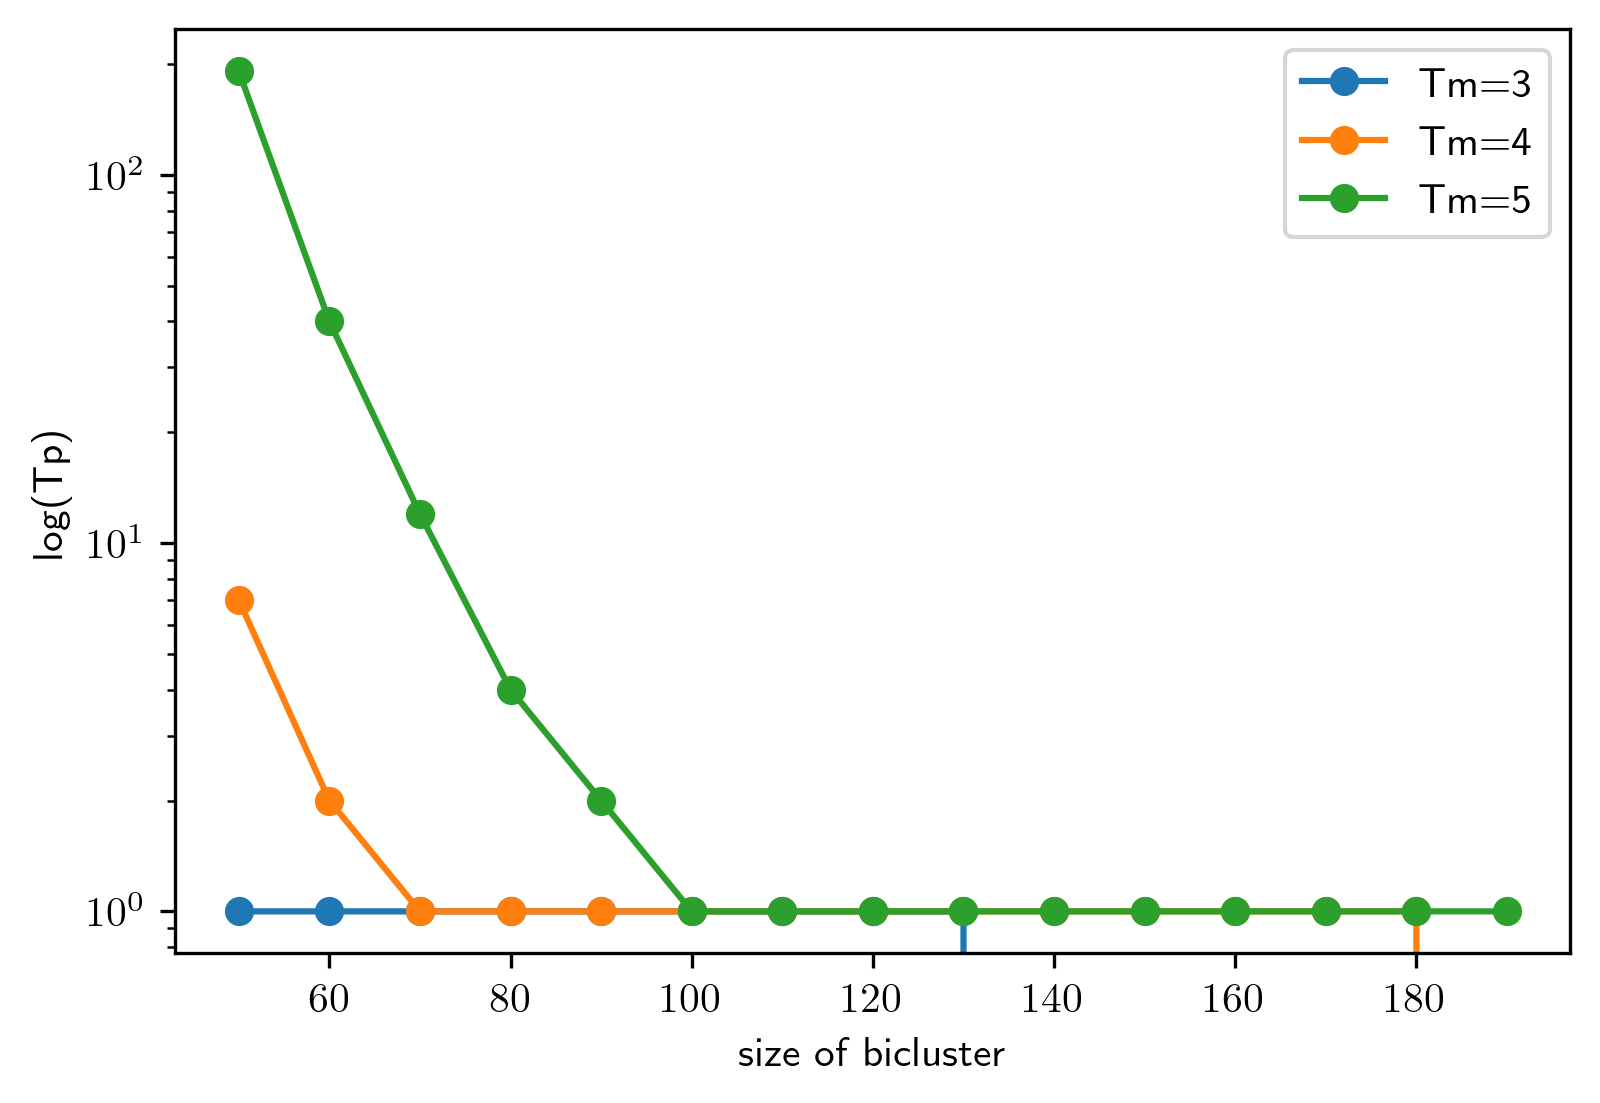
\includegraphics[width=\linewidth]{Tp.png}
                    \caption{Decide $T_p$}
                    \label{fig:image2}
                \end{subfigure}
                \vspace{-0.8cm}
                % \caption{Probability Model}
                % \label{fig:comparison}
            \end{figure}
        \end{column}
    \end{columns}

\end{frame}

% application
% 1. partition thus small memory requirement, so good to handle big data with parallel computing, thus NLP is a good application
% 2. partition can lead to batch stream processing, thus good for real-time data processing, thus stream data (e.g. stock price and recommendation system) is a good application

\section{Application}
\begin{frame}
    \frametitle{Application}
    \begin{itemize}
        \item \textbf{Big Data and NLP:} Partitioning allows for smaller memory requirements, making it highly efficient for handling big data. This is particularly useful in parallel computing environments. Natural Language Processing (NLP) can greatly benefit from this, as it often involves processing large datasets like text corpora or social media feeds \cite{affeldt2020EnsembleBlockCoclustering}

        
        \item \textbf{Real-Time Data Processing:} Partitioning is also conducive for batch stream processing. This is advantageous for real-time data processing applications. For instance, stream data such as recommendation systems can be processed in real-time, allowing for quicker decision-making and analytics \cite{zheng2017SupervisedAdaptiveIncremental}
    \end{itemize}
    % reference report.bib
    \scriptsize
    \bibliographystyle{plain}
    \bibliography{report}
\end{frame}



\end{document}